% % conventions:
% % crossrefs - typechap:name (type: [s]ection,[e]quation,[d]efinition,[t]heorem(lemma,..))
% %                           (chap: [p]hysical background, [m]ath tools, [f]luid, [b]odies, [s]teady)
% \documentclass[a4paper]{article}
% % ***************************************** PACKAGES
% \usepackage{amsmath}
% \usepackage{amsfonts}
% \usepackage{amssymb}
% \usepackage{amsthm}
% \usepackage{fancyhdr}
% \usepackage{graphicx}
% \usepackage[numbers]{natbib}
% 
% % ***************************************** SYMBOLS
 \def\abs#1{\lvert#1\rvert}
 \def\argdot{{\hspace{0.18em}\cdot\hspace{0.18em}}}
 \def\avg#1{\left\{#1\right\}}
 \def\D{{\tn D}}
 \def\div{\operatorname{div}}
 \def\Eh{\mathcal E_h}       % edges of \Th
 \def\Ehb{\mathcal E_{h,B}}  % edges of \Th on boundary
 \def\Ehcom{\mathcal E_{h,C}}         % edges of \Th on interface with lower dimension
 \def\Ehdir{\mathcal E_{h,D}}         % Dirichlet edges of \Th
 \def\Ehint{\mathcal E_{h,I}}       % interior edges of \Th
 \def\grad{\nabla}
 \def\jmp#1{[#1]}
 \def\n{\vc n}
 \def\vc#1{\mathbf{\boldsymbol{#1}}}     % vector
 \def\R{\mathbb R}
 \def\sc#1#2{\left(#1,#2\right)}
 \def\Th{\mathcal T_h}       % triangulation
 \def\th{\vartheta}
 \def\tn#1{{\mathbb{#1}}}    % tensor
 \def\Tr{\operatorname{Tr}}
 \def\wavg#1{\avg{#1}_\omega}
 \def\where{\,|\,}
% %***************************************************************************
% 


% \begin{document}


\chapter{Numerical methods}

In this chapter we briefly describe numerical methods used in Flow123d for solution of physical models
presented in Chapter \ref{PhysicalModels}. For the steady or unsteady Darcy flow we use mixed-hybrid discretization using Raviart-Thomas finite elements
described in details in Section \ref{MHmethod}.
For the numerical approximation of the advection-dispersion equation \eqref{e:ADE} we distinguish whether the dispersion $\D$ is present or not.
Since the true solution has qualitatively different properties, we also choose different numerical methods for each case. For purely advection problems
(i.e. without dispersion term) one can use finite volume method with up--winding and explicit Euler method fully described in Section \ref{Convection}.
For problems with dispersion term (even advection dominated) we provides implicit discontinuous Galerkin method covered in Section \ref{DGmethod}.


\section{Mixed-Hybrid method for Darcy flow (TO BE DONE)}
\label{MHmethod}
Based on publications: \cite{arbogast_nonlinear_1996}, \cite{maryska_mixed-hybrid_1995}, \cite{maryska_schur_2000}, \cite{vohralik_mixed-hybrid_2000}, \cite{VogelBrezina2010},
\cite{GerkeGenuchten1993a}, \cite{brezina_mixed-hybrid_2010}



\section{Pure advection (NEEDS ACTUALIZATION)}
\label{Convection}
% Copyright (C) 2007 Technical University of Liberec.  All rights reserved.
%
% Please make a following refer to Flow123d on your project site if you use the program for any purpose,
% especially for academic research:
% Flow123d, Research Centre: Advanced Remedial Technologies, Technical University of Liberec, Czech Republic
%
% This program is free software; you can redistribute it and/or modify it under the terms
% of the GNU General Public License version 3 as published by the Free Software Foundation.
%
% This program is distributed in the hope that it will be useful, but WITHOUT ANY WARRANTY;
% without even the implied warranty of MERCHANTABILITY or FITNESS FOR A PARTICULAR PURPOSE.
% See the GNU General Public License for more details.
%
% You should have received a copy of the GNU General Public License along with this program; if not,
% write to the Free Software Foundation, Inc., 59 Temple Place - Suite 330, Boston, MA 021110-1307, USA.

\normalsize
 \subsection{Advection-Diffusion equation}
 
Solute transport is governed by advection equation which can be written in the form
\begin{equation}
 \frac{\partial c}{\partial t} + \boldsymbol{v} \frac{\partial c}{\partial x}  = 0, \label{Aeq}
\end{equation}
where $c$ is concentration $[M^3 \cdot L^{-3}]$, $t$ is time $[T]$, $v$ is velocity $[L \cdot T^{-1}]$, and $x$ is coordinate in cartesian system $[L]$.
Assuming solution which is constant on every element (cell centered finite volume method) and integrating equation (\ref{Aeq}) we get
    \begin{equation}
    \int\limits_{e_i} \frac{\partial c}{\partial t} dV + \int\limits_{e_i} \boldsymbol{v} \frac{\partial c}{\partial x} \, dV = 0. \notag 
    \end{equation}
    After some rearrangements we obtain on $i$-th element ($e_i$)
    \begin{equation}
    \frac{\partial c_i}{\partial t}  V_{i} + c \int\limits_{\partial e_i }  \boldsymbol{v} \, \mathbf{dS} = 0, \label{Aeqint} 
    \end{equation}
  where $c_i$ is average concentration in $e_i$ and $V_{i}$ its volume, $c$ will be specified later (there are two main possibilities - $c_i$ or concentration from neighbouring element).
    Term $\frac{\partial c}{\partial t}$ we approximate by explicit Euler difference
    \begin{equation}
     \frac{\partial c}{\partial \textrm{t}} \approx \frac{c_{i}^{n+1} - c_{i}^n}{\Delta t}. \label{expliciteuler}
    \end{equation}
    Where $\Delta t$ is a time step and upper index at $c_i$ means values in the discrete time steps $n+1$ and $n$.
    We assume that all elements have piecewise smooth element boudary $\partial e$ with outwards directed normal. Inside the area $\Omega$ we introduce internal flows.
    With respect to $e_i$, we define internal flow intake $U_{ij}^{-}$ (from element $e_j$) and
    internal flow drain $U_{ij}^{+}$ (to element $e_j$) as follows
    \begin{eqnarray}     
      U_{ij}^{-} = \text{min}(\int\limits_{\partial e_i \cap \partial e_j, i \ne j} \boldsymbol{v} \, \mathbf{dS},0), \notag \\
      U_{ij}^{+} = \text{max}(\int\limits_{\partial e_i \cap \partial e_j, i \ne j} \boldsymbol{v} \, \mathbf{dS},0). \label{iflux}  
    \end{eqnarray}
  Those flows realizes solute transport in the area $\Omega$. On the $\partial\Omega$ we define external flows which will be important for transport Dirichlet boundary  
  conditions. In the same way as for internal flows we assume
  (with respect to element $e_i$) external flow intake $U_{ij}^{e-}$ (from $\partial\Omega$) and external flow drain $U_{ij}^{e+}$ (to $\partial\Omega$).
    \begin{eqnarray}     
      U_{ik}^{e-} = \text{min}(\int\limits_{\partial e_i \cap \partial \Omega } \boldsymbol{v} \, \mathbf{dS},0), \notag \\
      U_{ik}^{e+} = \text{max}(\int\limits_{\partial e_i \cap \partial \Omega } \boldsymbol{v} \, \mathbf{dS},0). \label{eflux}  
    \end{eqnarray}
    Direction of the velocity $\boldsymbol{v}$, which affects sign of the $U$-terms is significant for the construction solution. For the solution
    stability it is suitable to use an upwind scheme, which can by written for finite difference on simple 1D geometry in the form
    \begin{eqnarray} 
      v>0 : \frac{\partial c}{\partial \textrm{x}} \approx \frac{c_{i}^n - c_{i-1}^n}{\Delta x},   \notag \\
      v<0 : \frac{\partial c}{\partial \textrm{x}} \approx \frac{c_{i+1}^n - c_i^n}{\Delta x}.   \label{upwind} 
    \end{eqnarray}
    This scheme can be interpreted as well as in finite volume method - in convection term one can get $c$ value opposite the flow of the quantity $\boldsymbol{v}$ direction.
      For every $e_i$ we introduce itemsets $\mathcal{N}_{i}, \mathcal{B}_{i}$ which contains indexes of neighbourging elements, local boundary conditions respectivelly.  
     Assuming upwind scheme, using (\ref{iflux}), (\ref{eflux}), and  (\ref{expliciteuler}) we can write solution of the equation (\ref{Aeqint}) 
    (relation between two consecutive time steps) on $e_i$ in the form 
    \begin{equation}
      c_i^{n+1} = c_i^n - \frac{\Delta t}{V_{i}} \left[ \sum_{j \in \mathcal{N}_{i}} \left[ U_{ij}^{+} c_i +  U_{ij}^{-} c_{j} \right] +
      \sum_{k \in \mathcal{B}_{i}}  \left[  U_{ik}^{e+} c_i +  U_{ik}^{e-} c_{B_{ik}} \right] \right]. \label{Aeqsol}
    \end{equation}
    Where $c_{B_{ik}}$ are values of Dirichlet boundary conditions which belong to $e_i$. Formula (\ref{Aeqsol}) can be rewritten into the matrix notation
    \begin{equation}
     \mathbf{c}^{n+1} = (\mathbf{I} + \Delta t \mathbf{A}) \cdot \mathbf{c}^{n} + \Delta t \mathbf{B} \cdot \mathbf{c_{B}}^{n} \label{AeqsolM}
    \end{equation}
  Where $\mathbf{c}$ is vector of $c_i^{n+1}$, $\mathbf{A}$ is a square matrix composed from $\frac{U_{ij}^{+}}{V_i}$, $\frac{U_{ij}^{-}}{V_i}$, and
  $\frac{U_{ij}^{e+}}{V_i}$. $\mathbf{B}$ is in general rectangular matrix composed from $\frac{U_{ij}^{e-}}{V_i}$ and $\mathbf{c_{B}}^{n}$ is  vector of Dirichlet
  boundary conditions.matrix definition. There is one stability condition for time step which is called Courant-Friedrich-Levy condition. 
  For the problem without sources/sinks it can be written as
  \begin{equation}
  \Delta t_{max} = \min_i \left( \frac{V_i}{ \sum\limits_{j}  U_{ij}^{+} + \sum\limits_{k}  U_{ik}^{e+} } \right) =
  \min_i \left( \frac{V_i}{ \sum\limits_{j} | U_{ij}^{-} | + \sum\limits_{k} | U_{ik}^{e-} | } \right). \label{cfl} 
  \end{equation}
  This condition has a physical interpretation, which can be understood as conservation law - volume that intakes/drains to/from element $e_i$ 
can not be higher then element volume $V_i$. From algebraical point of view this condition can be seen as a condition which bounds norm of the evolution operator as follows 
  \begin{equation}
  \| \mathbf{I} + \Delta t \mathbf{A} \quad \Delta t \mathbf{B} \| \le 1.
  \end{equation}
 \subsection{Generalization}
  This approach can be used as well as for more general element connections -- for compatible/non-compatible element interconnection, if we know the flow integral
  values ($U_{ij}^{+}$ or $U_{ij}^{-}$). %Situation for more general case is in the picture (\ref{compmodel}).
      \begin{figure}[h]
        \begin{center}
        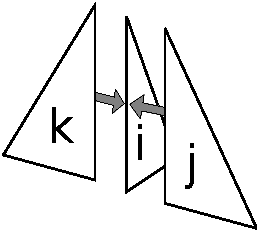
\includegraphics[scale=0.7]{obr7.pdf} 
	\caption{Edge with 3 elements}
	\label{edgemodel}
        \end{center}
      \end{figure}  
  The most general case of connection is relation among $n$ elements like in figure (\ref{edgemodel}). For this case we define
edge element indexset $\mathcal{G}_{l}$ that contains all the indexes of elements which sides make $l$-th edge ($g_l$), so that $\mathcal{G}_{l} = \{i,j,k\}$.
For $\mathcal{G}_{l}$ we introduce its subsets $\mathcal{G}_{ij}$, $\mathcal{G}_{ji}$, $\mathcal{G}_{ik}$, $\mathcal{G}_{ki}$, $\mathcal{G}_{kj}$, and $\mathcal{G}_{jk}$,
  where $\mathcal{G}_{ij} = \mathcal{G}_{ik} =  \mathcal{G}_{l} \backslash {i} = \{j,k\}$, $ \mathcal{G}_{ji} = \mathcal{G}_{jk} = \mathcal{G}_{l} \backslash {j} =\{i,k\}$, and
 $\mathcal{G}_{ki} = \mathcal{G}_{kj} = \mathcal{G}_{l} \backslash {k} =\{i,j\}$. It can be written in the same way for any edge $g$ with more than 3 elements, 
it is hold  $|\mathcal{G}_{g}| - 1 = |\mathcal{G}_{ab}|; \forall a,b \in \mathcal{G}_{g}$.
For $l$-th edge ($g_l$) we can define total edge flow $U_{g_{l}}$ eg. as
  \begin{eqnarray}
   U_{g_{l}} &=& \sum\limits_{m \in \mathcal{G}_{ji}}   \left[ U_{mj}^{+}   + \frac{ U_{jm}^{+}}{|\mathcal{G}_{ji}|} \right] = \sum\limits_{m \in \mathcal{G}_{jk}}  \left[ U_{mj}^{+}   +  \frac{ U_{jm}^{+}}{|\mathcal{G}_{jk}|} \right] \notag \\
	      &=& \sum\limits_{m \in \mathcal{G}_{ij}}  \left[ U_{mi}^{+}   +  \frac{ U_{im}^{+}}{|\mathcal{G}_{ij}|} \right] = \sum\limits_{m \in \mathcal{G}_{ik}} \left[  U_{mi}^{+} +  \frac{ U_{im}^{+}}{|\mathcal{G}_{ik}|} \right] \notag \\ 
	      &=& \sum\limits_{m \in \mathcal{G}_{ki}}  \left[ U_{mk}^{+}   +  \frac{ U_{km}^{+}}{|\mathcal{G}_{ki}|} \right] = \sum\limits_{m \in \mathcal{G}_{kj}}  \left[ U_{mk}^{+}   +  \frac{ U_{km}^{+}}{|\mathcal{G}_{kj}|} \right], \label{edgeflow}
  \end{eqnarray}
$U_{g_{l}}$ with respect to any $e_m$; $m \in \mathcal{G}_{l}$ has to have the same value because continuity equation, for assumed incompresible flow, has to
 be fulfilled in every edge. Edges with more than two elements and two and more nonzero intakes to edge realize an ideal mixing (to an average concentration) 
with weights which will be specified later. This fact modifies equation (\ref{Aeqsol}) on the general mesh into the form
    \begin{equation}
      c_i^{n+1} = c_i^n - \frac{\Delta t}{V_{i}} \left[ \sum_{j \in \mathcal{N}_{i}} \left[ U_{ij}^{+} c_i +  \frac{U_{ij}^{-}}{ \sum\limits_{k \in \mathcal{G}_{ij}}
      \left[ U_{ki}^{+} + \frac{U_{ik}^{+}}{|\mathcal{G}_{ij}|} \right] } \sum\limits_{k \in \mathcal{G}_{ij}} U_{ki}^{+} c_{k} \right] + 
      \sum_{k \in \mathcal{B}_{i}}  \left[  U_{ik}^{e+} c_i +  U_{ik}^{e-} c_{B_{ik}} \right] \right]. \label{Aeqsol2}
    \end{equation}
The edges with total edge flow $U_{g_{l}} = 0$ can occur breakdown in the equation (\ref{Aeqsol2}) via term $\sum\limits_{k \in \mathcal{G}_{ij}}\left[ U_{ki}^{+} + \frac{U_{ik}^{+}}{|\mathcal{G}_{ij}|} \right] = 0$.
This fact implies as well as numerator $U_{ij}^{-} = 0$. In order to avoid dividing by zero we have to assume computation only for nonzero flows.
Concentrations $c_k$, $k \in \mathcal{G}_{ij}$ that may intakes into element $e_i$ are weighted with weights 
\begin{equation}
 \alpha_k = \frac{U_{ki}^{+}}{\sum\limits_{k \in \mathcal{G}_{ij}} \left[ U_{ki}^{+} + \frac{U_{ik}^{+}}{|\mathcal{G}_{ij}|} \right] }, \label{weights}
\end{equation}
so that the ideal mixing in this edge leads to the average concentration 
\begin{equation}
 c_{av} = \frac{\sum\limits_{k \in \mathcal{G}_{ij}} U_{ki}^{+} c_{k}}{\sum\limits_{k \in \mathcal{G}_{ij}} \left[ U_{ki}^{+} + \frac{U_{ik}^{+}}{|\mathcal{G}_{ij}|} \right] }. \label{cav}
\end{equation}
Matrix notation is the same as in (\ref{AeqsolM}). Finally ...

\section{Advection with dispersion}
\label{DGmethod}

For the general case we use the discontinuous Galerkin space approximation described in \cite{ern_stephansen_zunino} and implicit Euler time discretization.
Let $\tau$, $h$ be the time step and the space discretization parameter, respectively.
We assume that $\Th^d$ is a regular partition of the domain $\Omega^d$ into simplices, $d=1,2,3$.
We define the set $\Eh^d$ of all edges of elements in $\Th$ (triangles for $d=3$, line segments for $d=2$ and points for $d=1$).
Further, $\Ehint^d$, $\Ehb^d$ will stand for interior and boundary edges, respectively, $\Ehdir^d(t)$ for edges that coincide with $\Gamma_D^d(t)$ and $\Ehcom^d$ for edges on interface with $\Omega^{d-1}$.

Let us fix one substance and the space dimension $d$.
At each time instant $t_k=k\tau$ we search for the concentration field $c_d^{h,k}\in V_d^h$, where
$$ V_d^h = \{v:\overline{\Omega^d}\to\R\where v_{|T}\in P_1(T)~\forall T\in\Th^d\} $$
is the space of functions piecewise affine on the elements of $\Th^d$, possibly discontinuous across the element interfaces.
The initial concentration $c^{h,0}_d$ is set to the projection of the initial data $c_0$ onto $V_d^h$.
For $k=1,2,\ldots$, the discrete problem reads:
\begin{equation*}
\sc{\delta^d\th\frac{c_d^{h,k}-c^{h,k-1}_d}\tau}{v}_{\Omega^d} + a^{h,k}_d(c^{h,k}_d,v) = b^{h,k}_d(v) \quad \forall v\in V^h_d.
\end{equation*}
Here $\sc{f}{g}_{\Omega^d}=\int_{\Omega^d} f g$, $c^{h,k-1}_d$ is the solution from the previous time step and the forms $a^{h,k}_d$, $b^{h,k}_d$ are defined as follows:
\begin{multline*}
a^{h,k}_d(u,v) = \sc{\delta^d\th\D\nabla u}{\nabla v}_{\Omega^d}
- \sc{\vc q u}{\nabla v}_{\Omega^d}\\
- \sum_{E\in\Ehint^d}\left(\sc{\wavg{\delta^d\th\D\nabla u}\cdot\n}{\jmp{v}}_E + \theta\sc{\wavg{\delta^d\th\D\nabla v}\cdot\n}{\jmp{u}}_E\right)\\
+ \sum_{E\in\Ehint^d}\sc{\vc q\cdot\n\avg{u}}{\jmp{v}}_E
+ \sum_{E\in\Ehb^d}\sc{\vc q\cdot\n u}{v}_E \\
+ \sum_{E\in\Ehint^d}\gamma_E\sc{\jmp{u}}{\jmp{v}}_E
+ \sum_{E\in\Ehdir^d(t_k)}\gamma_E\sc{u}{v}_E,
\end{multline*}
% 
\begin{equation*}
b^{h,k}_d(v) = \sum_{E\in\Ehdir^d(t_k)}\gamma_E\sc{c_D}{v}_E.
\end{equation*}
For an interior edge $E$ we denote by $T^-(E)$ and $T^+(E)$ the elements sharing $E$.
By $\n$ we mean the unit normal vector to $E$ pointing from $T^-(E)$ towards $T^+(E)$, the inter-element jump is defined as $\jmp{f}=f_{|T^-(E)}-f_{|T^+(E)}$, $\avg{f}=\frac12(f_{|T^-(E)} + f_{|T^+(E)})$ and $\wavg{f}=\omega f_{|T^-(E)} + (1-\omega) f_{|T^+(E)}$ denotes the usual and weighted average of the quantity $f$.
The weight $\omega$ is chosen in a specific way (see \cite{ern_stephansen_zunino} for details) taking into account possible inhomogeneity of $\D$.
The stabilization parameter $\gamma_E>0$ is user dependent; its value affects the inter-element jumps of the solution.
The constant $\theta$ can take the value $-1$, $0$ or $1$, which corresponds to the nonsymmetric, incomplete and symmetric variant of the interior penalty DG method.

% \paragraph{Communication between regions of the same dimension.}
In case that lower dimensional domains ($\Omega^1$, $\Omega^2$) have complex topology, e.g. if there are more triangles sharing one line segment, then we consider ideal mixing, i.e. the concentration entering the edge through every inlet element ($\vc q$ points out of this element) is divided among all outlet elements proportionally to their fluxes.

If there are interfaces between adjacent dimensions, then the following terms are added to the bilinear forms:
\begin{multline*}
a^{h,k}_{d+1,C}((u_{d+1},u_d),v_{d+1})\\
= \sum_{E\in\Ehcom^{d+1}} \sc{\delta_{d+1}\sigma^c(\th_{d+1}u_{d+1}-\th_d u_d)+(\vc q\cdot\n)^+u_{d+1} - (\vc q\cdot\n)^-u_d}{v_{d+1}}_E,
\end{multline*}
\begin{multline*}
a^{h,k}_{d,C}((u_{d+1},u_d),v_d)\\
= -\sum_{E\in\Ehcom^{d+1}} \sc{\delta_{d+1}\sigma^c(\th_{d+1}u_{d+1}-\th_d u_d)+(\vc q\cdot\n)^+u_{d+1} - (\vc q\cdot\n)^-u_d}{v_d}_E.
\end{multline*}
Here $f^+=\max\{0,f\}$ and $f^-=-\min\{0,f\}$ is the positive, negative part, respectively and $\Ehcom^4=\Ehcom^1=\emptyset$.

A priori error estimates for the equation in a single domain are done in \cite{ern_stephansen_zunino}, for a posteriori estimates see \cite{ern2010guaranteed}.

% TODO:
% \begin{itemize}
%   \item Write equations for sorption and integrate them into \eqref{e:ADE}. 
% $R_i(\argdot)$ is a ``retardation function'' its a function which includes various types of equilibrium sorption.
% It is in general dependent as on the substance $i$ as on the material in particular location in space. 
% 
% \end{itemize}
% 
% 
% 
% 
% \begin{enumerate}
%  \item Explicit solution - technicaly this is only slight modification of the already implemented transport model. One has to add appropriate 
%        diffusive flux approximation. Something was done by Sembera nad Jiranek, however there are more possible approximations (further search). Weakness:
%        \begin{itemize}
%         \item too restrictive condition on timestep size for big diffusion on small elements
% 	      \[
% 	         dt \le \min \frac{dx^2}{2D},\qquad dt\le \min \frac{dx}{v}
% 	      \]
% 	\dots so the former condition is more restrictive if $\min dx / D \le 2\min 1/v$ \dots Peclet number can not be used since it 
%         measure only local balnace between diffusion and convection
% 
%         \item persisting problems with CFL condition
%         \item problems with approximation of the diffusive flux with anisothropy raising from the dispersion
%        \end{itemize}
%   \item Implicit solution
%   \begin{enumerate}
%        \item Finite volumes/ Discontinuous Galerkin - search for suitable approximation of the diffusive flux (as above)
%        \item Lumped MH  for diffusion, upwind for convection. Problem with zero or nearly zero $\tn D$. There has to be also implementation without
%              diffusion (no whole MH stuff). Problem that with lumping this leads to edge centered finite volumes.
%   \end{enumerate}   
%   
% \end{enumerate}



%\bibliographystyle{abbrvnat}
%\bibliography{flow123d_doc}


%\end{document}
